The value in the resampling process above largely lies in the ability to present well-defined document prototypes to a retrieval stage.  There are many potential sources for document retrieval according to this prototype, including the original input corpus, a separate `super-corpus', or, ideally a separate population (that is itself not a sample).



\subsection{Method}
\label{sec:evaluation:method}

The proof-of-concept evaluated here implements a mechanism similar to that of BootCaT~\cite{baroni2004bootcat}, using a search engine to retrieve results based on key n-grams.  This mechanism was selected due to the pertinence of its method to other corpus building efforts---there is no technical limitation imposed by the software tool, and users are free to select any other source of data or mechanism of retrieval.

The similarity of the retrieval system described here to BootCaT, along with the use of concrete prototype documents, allows us to inspect the `measurement error' of using search engines to retrieve data based on key terms.  This evaluation is, therefore, primarily an assessment of that bias and a preliminary assessment of its sources.

% ---

\begin{figure}[Ht]
    % ./analysis/loglik-significance.r
    \centering
    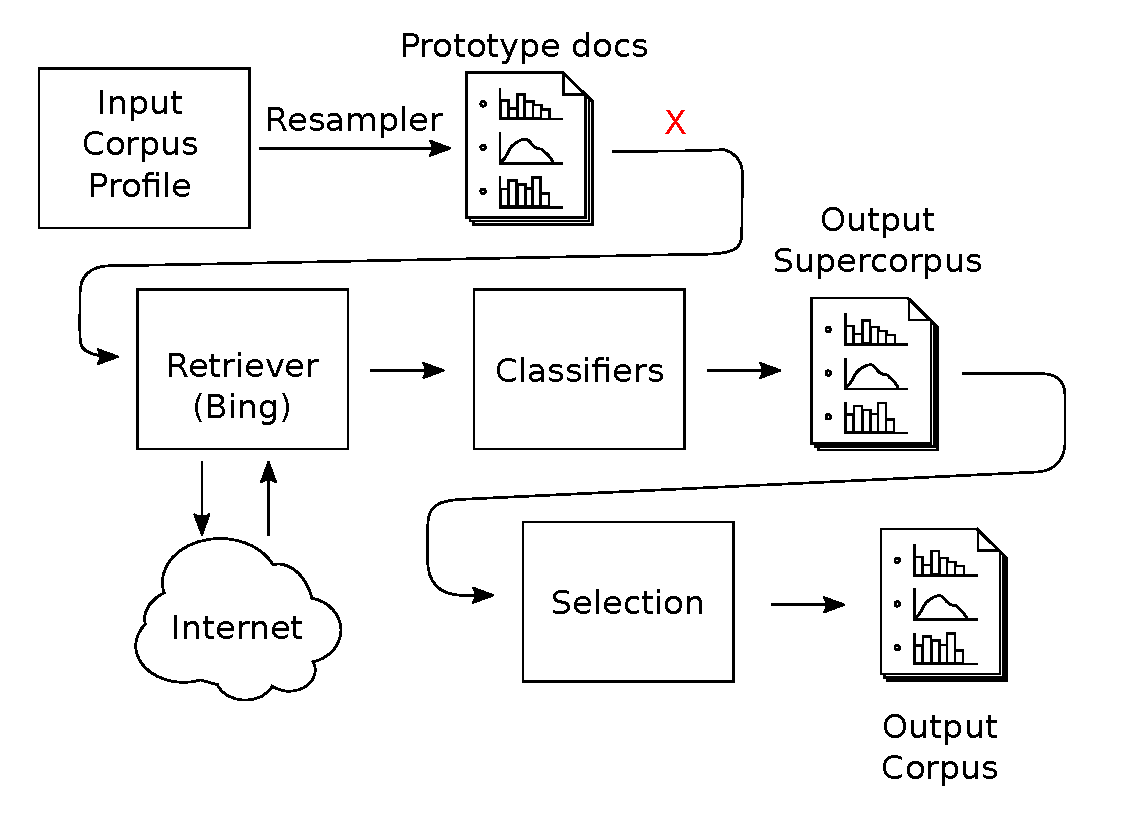
\includegraphics[width=0.9\textwidth]{evaluation/retrieval-overview}
    \caption{An overview of the retrieval mechanism used in the proof-of-concept implementation.}
\label{fig:evaluation:retrieval:outline}
\end{figure}


The retrieval process (as summaried in Figure~\ref{fig:evaluation:retrieval:outline}) is performed iteratively using the components evaluated in the previous sections:

\begin{enumerate}
    \item Sample a prototype document from the corpus profile;
    \item Retrieve candidate links using the Microsoft Bing search engine\footnote{\url{https://datamarket.azure.com/dataset/bing/searchweb}};
    \item Download, remove boilerplate (using JusText~\cite{pomikalek2013justext}), and classify each document using heuristics from the corpus profile;
    \item Measure distance in the resulting vector space according to each heuristic's value.
\end{enumerate}

For this data set, both the direct links from Bing and the first level of hyperlinks in each document were downloaded.  Spidering was performed in order to ensure that the sampled area of metadata is a supersample of the desired distribution, as well as to maximise the chances of finding suitable points in other, uncontrolled, dimensions.

Documents with fewer than 100 words were discarded as they were unlikely to be classified accurately.  This could be worked around by selecting 100-word samples from larger texts if necessary.

For this evaluation, the written portions of the BNC were used as the seed corpus.  Keywords used for search were generated using log likelihood scores, and no cutoff was used: instead, the random selection algorithm was weighted by the resulting score.

The spoken and \texttt{W\_Misc} categories were omitted for a number of reasons.  Spoken data was omitted on the conjecture that it is difficult to find online~\footnote{Retrieval of transcriptions may be facilitated by searching for genre-specific features in addition to keywords, and this form of specialism is a potential avenue for improving the accuracy of all genres.}, leading to a predictable gap in the resulting corpus.  \texttt{W\_misc} was omitted due to the need for an accurate classification step, and because keyword-based retrieval requires that said keywords are highly representative of a given genre.  Both of these issues are potentially solvable in future work, yet lie outside the scope of this thesis.


The retriever must, as far as possible, return documents according to \textsl{all} prototype metadata dimensions, that is, it must perform the equivalent to an agglomerative query.  This is a particular challenge for search engines due to their generality.  Since the Bing API lacks tools to filter by any of the three dimensions used in this evaluation, the primary focus was on genre---word count and reading ease were both free to vary.  Language was specified as \texttt{en\_GB}.

% TODO: Write in discussion about how this is challenging but that a hybrid system might work best, say retrieve from scholar if it's a paper.









% This process is deliberately agnostic of any internal variables: the \textsl{content} of the retrieved texts is also affected by the choice of retrieval mechanism, however, this is part of the variance desired in the dataset, and should form part of any motivating research question.

% The problem of when the output corpus is `sufficiently large' may not be solved using this method: whilst the convergeance of the output corpus to the input is known to some degree of certainty, the same cannot be said of the errors in retrieval.  Assuming that each text is entirely accurate to its prototype will yield a corpus showing the same distribution as the input, but this does not mean that the source used is presenting data in an unbiased manner, or that sufficient variation has been captured to generalise about \textsl{that} population.

% It is also possible to select documents that are not a perfect fit to the prototype: indeed, this may be necessary where continuous measures are used to characterise the sampling design.  In this case, the residual variation may be used to determine bias in the selection method by measuring how non-uniform the distribution of these residuals is.  Note, however, that even uniform nonzero residuals represent an overall increase in dispersion compared to the input distribution: it is almost certainly more useful to deliberately apply this to the input distribution by applying a smoothing method prior to resampling than it is to rely on the document retrieval stage (which may apply said dispersion in less predictable ways).

% \til{
% further work:\\
% Though not implemented here, it is possible to use this known error distribution as a correction mechanism for the sampler, deliberately seeking to `shore up' the residuals.  This kind of feedback loop is used in bootstrapping algorithms such as Gibbs and slice sampling, though its application to a procedure based on a fairly hard-to-predict search mechanism (web search engines) presents major engineering challenges.
% }

% % --



% The retrieval method used here (outlined in Chapter~\ref{sec:rebuilding} and Figure~\ref{fig:evaluation:retrieval:outline}) is based on the principle of heuristically seeking documents fitting the prototype, followed by a ranking stage and selection of the highest-ranked document.  This means that it has the potential to output imperfect documents but is maximally unlikely to do so.  It does not adjust for any accumulated error during execution, so has the potential to gradually accumulate errors in one particular direction if `perfectly matched' documents are not available within the parameters given.  This approach is largely taken to prevent the retriever from searching endlessly for a combination of metadata values that simply do not exist in the sources to which it has access: many specific uses of this technique will be able to use far more certain methods for their retrieval stage (up to and including manual selection of documents).








\subsection{Results}
\label{sec:evaluation:results}

In total $72,540$ documents were downloaded after $6,510$ requests to Bing.  After boilerplate removal using JusText~\cite{pomikalek2013justext} and discarding of short documents, $55,790$ documents remained in the corpus.


This sample size is $\approx 21$ times the input corpus.  Estimating using graphical methods (as in Section~\ref{sec:evaluation:resampler}, this should be sufficient to provide an appropriately distributed sample of genres.  The worst case is that each Bing search returns very few documents with the desired genre, for example, if each search returns only a single document of interest then this ratio is reduced to $\approx 3n$.



% \subsubsection{Univariate Properties}
Before inspecting the results from the retriever, the limitations of this method should be noted.  Firstly, the ideal retrieval mechanism should target all dimensions of the prototype document provided, in this case Genre, reading ease, and word count).  Bing does not index the latter of these two, leaving them to vary naturally.

This variation interacts with the genre itself, and so it is not possible to generalise from the observations here to the wider web.  The distributions shown in Figures~\ref{fig:evaluation:retrieval:flesh} and~\ref{fig:evaluation:retrieval:words} are, however, indicative of the documents found via Bing when searching for BNC terms.  Upholding the assumption that the written BNC represents general-purpose language use, this is an indication of users' exposure to documents online.%\footnote{This is a distinction drawn strongly amongst WaC, where many efforts attempt to describe the web itself rather than usage thereof.}.

From the point of view of one sampling documents to form a supercorpus, it is desirable that the uncontrolled dimensions are widely and evenly dispersed across the vector space, such that any subsequent rejection sampling is simplified.


\begin{figure}[Ht]
    % ./analysis/
    \centering
    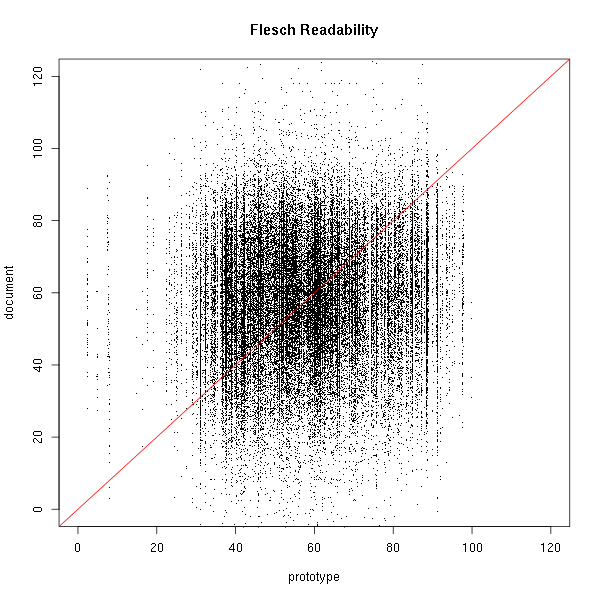
\includegraphics[width=0.8\textwidth]{evaluation/retrieval-flesch}
    \caption{Prototype/document readability scores}
    \label{fig:evaluation:retrieval:flesh}
\end{figure}

\begin{figure}[Ht]
    % ./analysis/
    \centering
    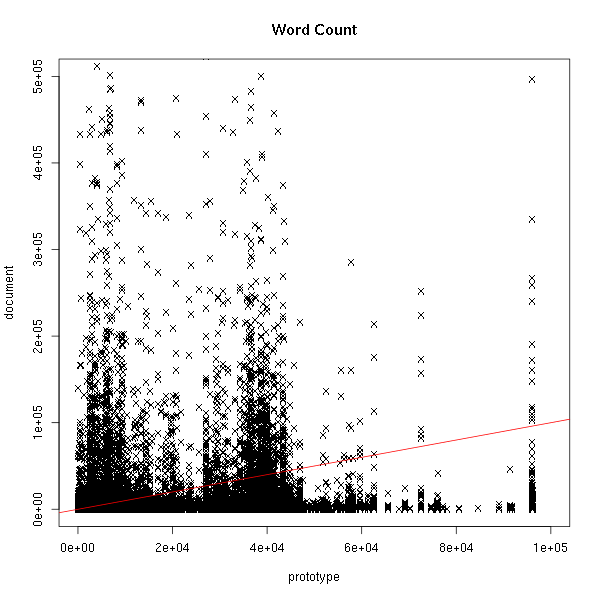
\includegraphics[width=0.8\textwidth]{evaluation/retrieval-words}
    \caption{Prototype/document word counts}
    \label{fig:evaluation:retrieval:words}
\end{figure}

Figure~\ref{fig:evaluation:retrieval:flesh} shows the distribution of reading ease scores across the collected documents, the $y$ axis showing the values as downloaded from the web.  The red line is plotted with a gradient of $0.5$, and shows the ideal zone where documents should lie if retrieved perfectly.


The readability dimension (Figure~\ref{fig:evaluation:retrieval:flesh}) is fairly well dispersed, indicating that there are no documents fundamentally unreachable using the search engine method.  Though this dimension is the simplest, both the prototype and retrieved documents have similar standard deviations ($16.2$ and $17.9$ respectively) and means ($57.5$ and $57.4$ respectively).  There is very little correlation between prototype and retrieved values: with a PMCC of just $0.06$.  Generally, this indicates that most distributions of readability are `covered' online, and the one used in the BNC is easily represented.

\begin{figure}[Ht]
    % ./analysis/
    \centering
    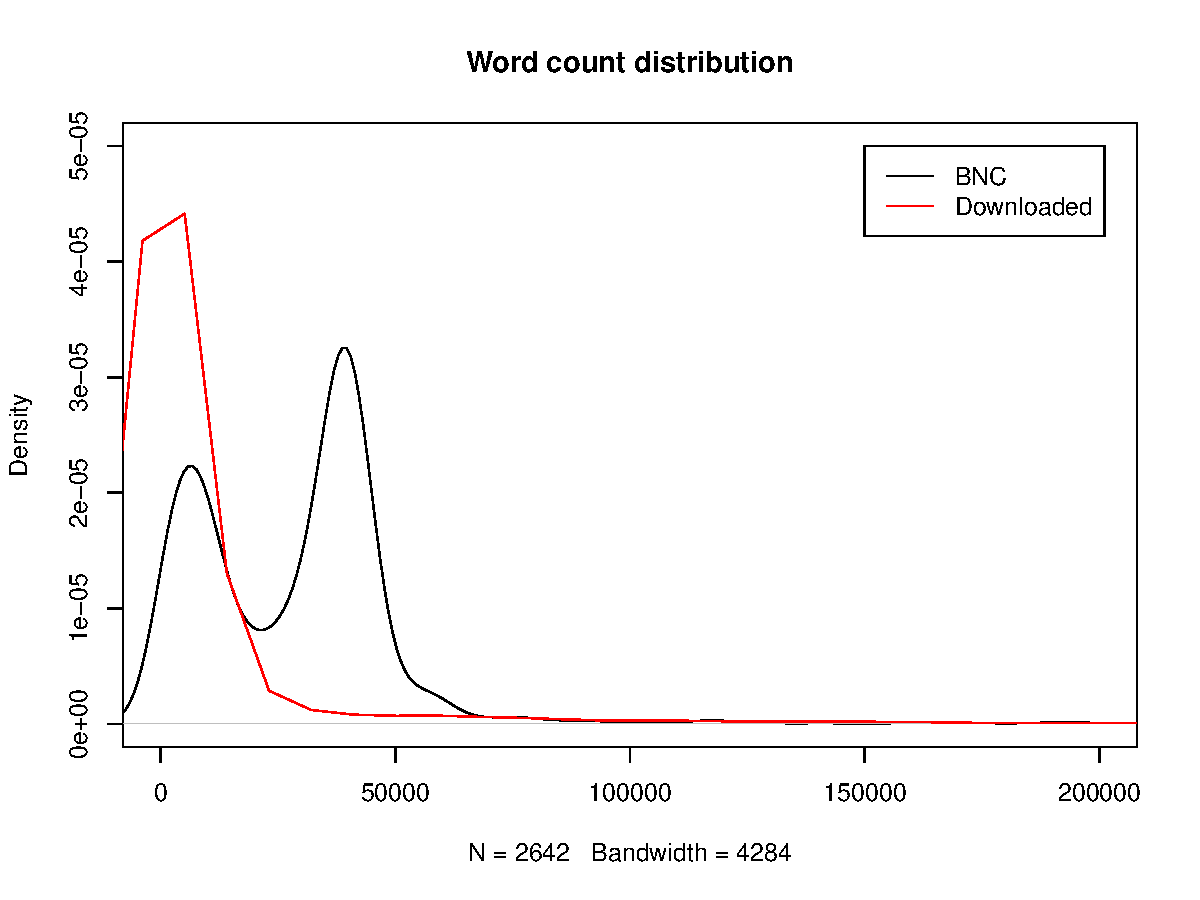
\includegraphics[width=0.8\textwidth]{evaluation/retrieval-words-dist}
    \caption{Distribution of document lengths in the written BNC and downloaded corpora}
    \label{fig:evaluation:retrieval:words-dist}
\end{figure}

Word counts are altogether more complex.  The word count is distributed in the BNC in a far more complex manner (Figure~\ref{fig:evaluation:retrieval:words-dist}), and the method of sampling can be reasonably expected to impact this more than readability.  This shows that the distribution of word counts online (conditioned on genre) is far from that in the BNC: the line of intended fit failing to intersect with longer documents.
% TODO

The distribution plots in Figure~\ref{fig:evaluation:retrieval:words-dist} display the obvious missing portion of the word count target distribution.  This is a clear example of the bias of online documents, which tend to be paginated even where the content is particularly long (a trend that is exacerbated by advertising-based funding models).  The bimodal distribution of the BNC's word counts can be attributed to interactions with `domain'%
%\td{define domain re. lee}\footnote{CHECK LEE's BNC COMMENTS ON DOMAIN}
: with \texttt{W\_world\_affairs} and \texttt{W\_imaginative} forming the bulk of the longer texts.

% \til{
% In the discussion section, mention that this bias can be worked around for most analysis by not sampling whole texts, but that it is an interesting finding that the web can't do long texts.  Perhaps refer to this in the keyword bit later.
% }



\begin{table}[Ht]
    \centering

    \begin{tabular}{|r|l|r|r|r|r|}
        \hline
        & Genre & Prototype & Downloaded & TP & tpr (\%) \\ 
        \hline
        1 & W\_ac\_humanities\_arts & 2180 & 1089 & 181 & 8.30 \\ 
        2 & W\_ac\_medicine & 987 & 1162 & 415 & 42.05 \\ 
        3 & W\_ac\_nat\_science & 684 & 1258 & 160 & 23.39 \\ 
        4 & W\_ac\_polit\_law\_edu & 4424 & 1467 & 590 & 13.34 \\ 
        5 & W\_ac\_soc\_science & 3112 & 1074 & 290 & 9.32 \\ 
        6 & W\_ac\_tech\_engin & 466 & 1267 & 129 & 27.68 \\ 
        7 & W\_admin & 195 & 1038 & 23 & 11.79 \\ 
        8 & W\_advert & 856 & 4501 & 273 & 31.89 \\ 
        9 & W\_biography & 2979 & 1736 & 221 & 7.42 \\ 
        10 & W\_commerce & 2952 & 2058 & 464 & 15.72 \\ 
        11 & W\_email &  46 & 882 & 3 & 6.52 \\ 
        12 & W\_essay\_school &   1 & 871 & 0 & 0 \\ 
        13 & W\_essay\_univ & 246 &  23 & 0 & 0 \\ 
        14 & W\_fict\_poetry & 815 & 460 & 42 & 5.15 \\ 
        15 & W\_fict\_prose & 10487 & 1844 & 888 & 8.47 \\ 
        16 & W\_hansard & 161 & 114 & 39 & 24.22 \\ 
        17 & W\_institut\_doc & 572 & 1952 & 131 & 22.90 \\ 
        18 & W\_instructional & 111 & 941 & 54 & 48.65 \\ 
        19 & W\_letters\_personal & 124 & 611 & 9 & 7.26 \\ 
        20 & W\_letters\_prof & 227 & 396 & 9 & 3.96 \\ 
        21 & W\_newsp\_brdsht\_nat\_arts & 764 & 3470 & 147 & 19.24 \\ 
        22 & W\_newsp\_brdsht\_nat\_commerce & 792 & 484 & 100 & 12.63 \\ 
        23 & W\_newsp\_brdsht\_nat\_editorial & 212 & 909 & 23 & 10.85 \\ 
        24 & W\_newsp\_brdsht\_nat\_misc & 1544 & 896 & 45 & 2.91 \\ 
        25 & W\_newsp\_brdsht\_nat\_report & 854 & 925 & 73 & 8.55 \\ 
        26 & W\_newsp\_brdsht\_nat\_science & 235 & 284 & 6 & 2.55 \\ 
        27 & W\_newsp\_brdsht\_nat\_social & 881 & 259 & 6 & 0.68 \\ 
        28 & W\_newsp\_brdsht\_nat\_sports & 639 & 503 & 97 & 15.18 \\ 
        29 & W\_newsp\_other\_arts & 216 & 1345 & 49 & 22.69 \\ 
        30 & W\_newsp\_other\_commerce &  91 & 466 & 18 & 19.78 \\ 
        31 & W\_newsp\_other\_report & 756 & 933 & 52 & 6.88 \\ 
        32 & W\_newsp\_other\_science & 327 & 196 & 3 & 0.92 \\ 
        33 & W\_newsp\_other\_social & 904 & 705 & 41 & 4.54 \\ 
        34 & W\_newsp\_other\_sports &  26 & 540 & 4 & 15.38 \\ 
        35 & W\_newsp\_tabloid &  45 & 482 & 2 & 4.44 \\ 
        36 & W\_news\_script & 479 & 121 & 3 & 0.63 \\ 
        37 & W\_non\_ac\_humanities\_arts & 1610 & 1665 & 193 & 11.99 \\ 
        38 & W\_non\_ac\_medicine & 384 & 1605 & 142 & 36.98 \\ 
        39 & W\_non\_ac\_nat\_science & 1438 & 1534 & 258 & 17.94 \\ 
        40 & W\_non\_ac\_polit\_law\_edu & 2891 & 1428 & 463 & 16.02 \\ 
        41 & W\_non\_ac\_soc\_science & 2210 & 1516 & 134 & 6.06 \\ 
        42 & W\_non\_ac\_tech\_engin & 2578 & 807 & 513 & 19.90 \\ 
        43 & W\_pop\_lore & 3371 & 6918 & 662 & 19.64 \\ 
        44 & W\_religion & 838 & 1942 & 400 & 47.73 \\ 
        \hline
    \end{tabular}


    \caption{Document counts by genre for prototypes and downloaded documents.}
    \label{table:evaluation:retrieval:words-dist}
\end{table}

\FloatBarrier{}

\begin{figure}[Ht]
    % ./analysis/
    \centering
    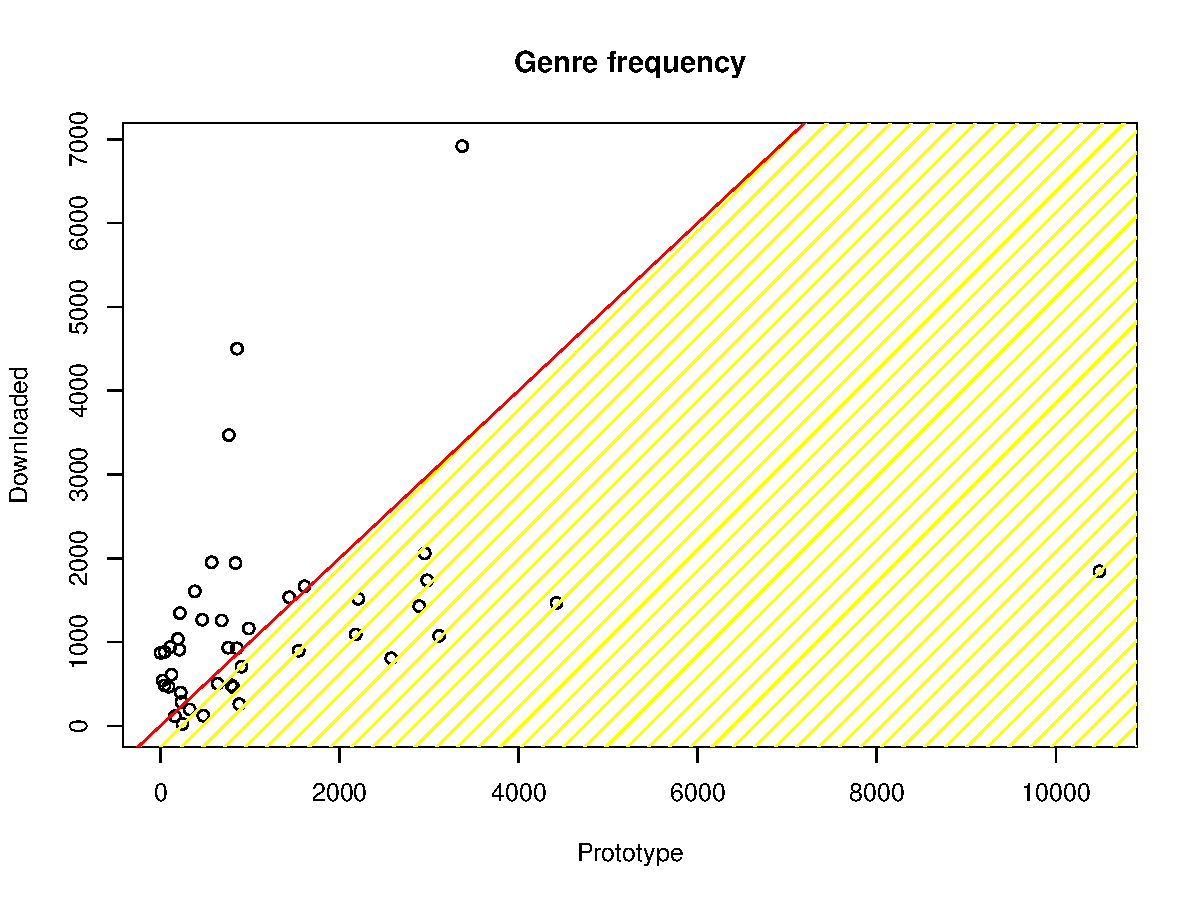
\includegraphics[width=0.8\textwidth]{evaluation/retrieval-genres-corr}
    \caption{Prototype genres frequencies and resulting downloaded document frequencies.  Shaded area indicates `over-downloaded' categories.}
    \label{fig:evaluation:retrieval:genres-corr}
\end{figure}


\begin{figure}[Ht]
    % ./analysis/
    \centering
    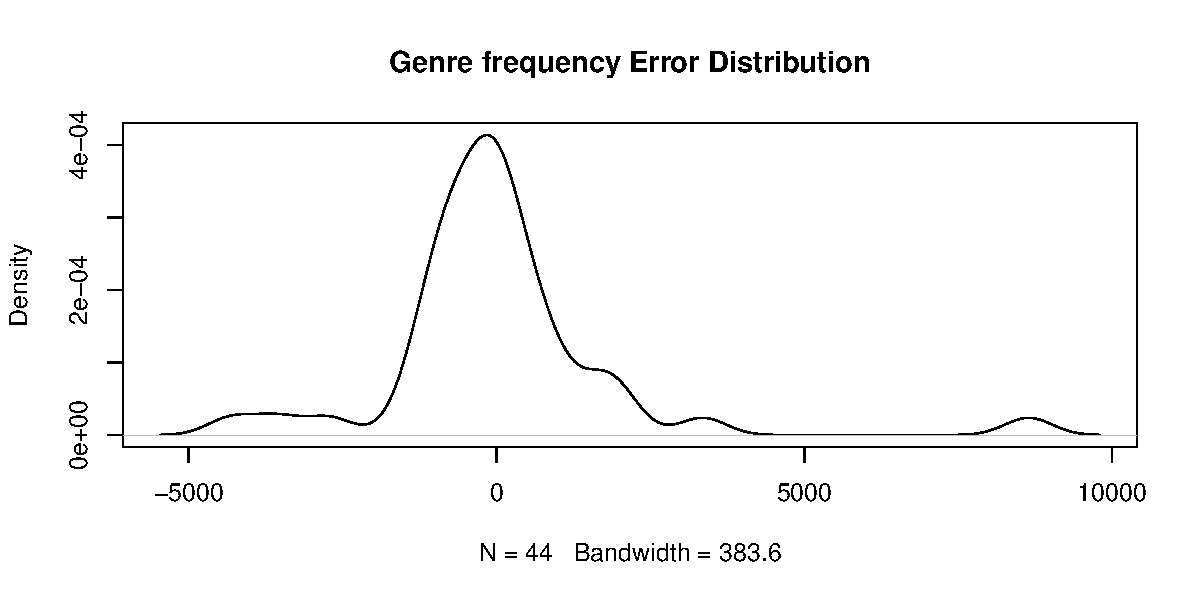
\includegraphics[width=0.8\textwidth]{evaluation/retrieval-genres-diffdist}
    \caption{The distribution of differences in genre frequency between prototype and downloaded documents.}
    \label{fig:evaluation:retrieval:genres-diffdist}
\end{figure}


Genre was the only parameter explicitly controlled-for by the search engine retrieval method.  Precise counts for each of the prototype and retrieved genres are provided in Table~\ref{table:evaluation:retrieval:words-dist}.  

Figure~\ref{fig:evaluation:retrieval:genres-corr} shows the prototype vs.\ downloaded genre frequencies.  Those genres above the line are under-represented in the downloaded documents, relative to the prototype documents\footnote{This measure is distinct from precision/recall in that it does not care which individual documents account for the frequencies, only that the search has retrieved appropriate proportions of each}.
When selecting a full corpus using the search engine lookup method, differences between the prototype and downloaded document classes should be minimal---when selecting a supercorpus, care must be taken to ensure that items in the top-left of the plot have sufficient frequencies for the intended purpose.
% In the ideal casejust $19$ of the $44$ categories have been "over-sampled".

Evidence for the `directedness' of genre-based retrieval using n-grams is given by the dispersion of data around the red line.  Rank correlation between prototype and retrieved documents is $0.45$, and a Mann-Whitney test is not significant ($U = 786.5; p \approx 0.13 > 0.05$), indicating that errors in retrieval are loosely centred around the prototype's frequencies.  This is reinforced by inspecting the density plot for differences between category frequencies, shown in Figure~\ref{fig:evaluation:retrieval:genres-diffdist}.
%This is evidence that retrieval using search terms produces documents similar to those searched for.

% --

Treating the searching process as a classifier allows us to examine the expectation of retrieving a genre successfully.  $7,355$ documents were returned with the desired genre, leading to a true positive rate of $13.2\%$.  This implies retrieval results close to the worst case of one relevant document per search, and explains the low correlation between predicted and resultant class types.  Note that the number of useful documents is above this thanks to re-examination of those previously returned.

Per-class retrieval rates are displayed in the right-most column of Table~\ref{table:evaluation:retrieval:words-dist}.  There is correlation between the size of a genre and its true positive rate ($\rho = 0.29$)%
% Spearman: rho = 0.59
% not sure what this is: ($\rho = 0.84$)
, and inspection of the table indicates that performance is better predicted by the `linguistic specificity' of a given category (with religion, medicine and tech leading the recall rate statistics).

Though it is not possible to separate classifier error from retrieval error without construction of a gold standard corpus (something that lies beyond the scope of this work), earlier evaluations of the classifier used (Section~\ref{sec:evaluation:heuristics:genre}) show that classifier error is not strongly biased.  This allows us to conclude that evidence of significant bias in the resultant data is largely a product of the searching process, rather than document classification.


% -- 



\begin{table}[hb]
    \centering
    \begin{tabular}{@{}llll||llll@{}}
        \hline
        \multicolumn{4}{c||}{{\bf Over-sampled}}                       & \multicolumn{4}{c}{{\bf Under-sampled}}                         \\ 
        {\bf term} & {\bf original} & {\bf retrieved} & {\bf loglik} & {\bf term}    & {\bf original} & {\bf retrieved} & {\bf loglik} \\ \hline
        p          & 29217          & 8839489         & 1977900.5    & she'd         & 7338           & 4050            & -17407.3     \\
        s          & 17778          & 1903037         & 357245.2     & darlington    & 5559           & 1521            & -16657.0     \\
        she        & 290860         & 916731          & 136365.1     & ec            & 6091           & 5531            & -11220.7     \\
        gt         & 111            & 535127          & 134335.1     & solicitors    & 2135           & 1086            & -5237.0      \\
        com        & 172            & 465891          & 116044.3     & swindon       & 2182           & 1409            & -4825.7      \\
        www        & 2              & 448772          & 113981.6     & kinnock       & 1375           & 264             & -4466.7      \\
        amp        & 668            & 432633          & 102780.7     & theda         & 838            & 32              & -3297.3      \\
        lt         & 792            & 425436          & 99921.8      & nizan         & 756            & 6               & -3146.1      \\
        had        & 359670         & 1439973         & 94877.1      & cnaa          & 742            & 1               & -3140.1      \\
        h          & 8094           & 555374          & 90772.7      & guil          & 755            & 43              & -2886.5      \\
        t          & 9078           & 557616          & 87217.1      & maastricht    & 1165           & 593             & -2856.9      \\
        her        & 277189         & 1070672         & 80897.8      & oesophageal   & 957            & 279             & -2820.0      \\
        2015       & 25             & 293434          & 74145.0      & lexical       & 1106           & 514             & -2809.1      \\
        2014       & 16             & 254997          & 64517.4      & robyn         & 1200           & 707             & -2767.5      \\
        he         & 523177         & 2629585         & 59109.8      & lamont        & 1184           & 708             & -2712.6      \\
        was        & 722425         & 3866921         & 58399.0      & risc          & 1013           & 416             & -2689.4      \\
        cent       & 34353          & 44410           & 49457.4      & knitting      & 1509           & 1463            & -2668.9      \\
        the        & 5021789        & 33346038        & 47673.9      & athelstan     & 1060           & 516             & -2645.3      \\
        be         & 524709         & 2771036         & 45819.9      & privatisation & 1104           & 665             & -2521.1      \\
        it         & 727487         & 4058706         & 45306.4      & leapor        & 626            & 18              & -2502.2      \\ \hline
    \end{tabular}

    \caption{The 20 most over- and under-represented terms relative to the BNC.}
    \label{table:evaluation:retrieval:keywords}

\end{table}






Finally, keywords were computed relative to the original input corpus using log likelihood.  These offer insight into the specific biases of the data source and a handle on qualitative differences between sampling processes.  

% This is a comparison of the supercorpus against the input used to generate it.
% Should a 'fake' BNC be generated by rejection sampling the supercorpus too?  The comparison would arguably be fairer.


The top 200 keywords\footnote{I recognise that nspection of the top $n$ keywords is not a hugely sound methodology, but it should prove indicative for these purposes} were inspected for the whole supercorpus relative to the seed corpus. Overrepresented tokens were scored separately to under-represented ones in accordance with Baron et.\ al.\cite{baron2009word}, and the lists were free-coded for prominent themes.  The 20 most over- and under-represented terms are displayed in Table~\ref{table:evaluation:retrieval:keywords}.  The full lists are included in Appendix~\ref{sec:appx:keywords}.

Overrepresented terms may be grouped into a number of categories.  The first of these is technical terms: those that are side-effects of the tokeniser or otherwise are related specifically to the web.  This includes features such as protocols (\textsl{HTTP}), and features of URLs (\textsl{co}, \textsl{org}), as well as terms such as \textsl{email} and \textsl{posted} which have simply become more prevalent since the BNC was produced.  It's difficult to say whether or not a more recent seed corpus would eliminate most of these from the keyword list.

Temporal features dominate the rest of the list, with many terms related to date or proper nouns (\textsl{Obama}, \textsl{Nike}).  Dates feature prominently: \textsl{2001}-\textsl{2012} are all mentioned, along with \textsl{1991} and \textsl{1988}.  Genetics is also mentioned (\textsl{gene}, \textsl{mutation}), along with education (\textsl{university}, \textsl{pupils}) and government (\textsl{government}, \textsl{council}).

The remaining terms are pronouns or function words.  These, along with the large number of quantities and references to time/date imply consistency with other WaC studies, that is, an overrepresentation of news online.

This central theme is interesting to contrast against the BNC, which contains a large quantity of news material already, indicating that news genres are even more prevalent online, or that news media (or perhaps just online news) has become more extreme (that is, less similar to other written genres) than the bulk of the BNC data.

Features that are significantly under-represented prodominantly fall into the category of proper nouns, and these are mostly political and from the UK (\textsl{Kinnock}, \textsl{Gummer}, \textsl{Heseltine}).  Since the search engine was instructed to search the `GB' marketplace, many of these are most likely explained by temporal effects---the prevalence of these keywords also points at the strength of news within the BNC, along with places and organisations that featured in the news at the time (\textsl{TUC}, \textsl{Maastricht}, \textsl{DTI}).

There is also a strong theme of legal terms (\textsl{offeror}, \textsl{solicitor}, \textsl{arbitrage}), which points at a clear under-representation of legal documents returned by search engines.  This is likely a technical limitation of the retriever, which avoids files in PDF format.

Some technical terms are also presented in the keyword list due to the speed of progress in that field: \textsl{80486} and \textsl{microcomputer} both showing their age.

Finally, there are a number of gastric terms (\textsl{oesophegeal}, \textsl{pylori}, \textsl{dueodenal}), which point to a very specific set of documents missing in the returned data.  These terms are from an academic context that, like legal documents, is under-represented for technical reasons, however, it is also likely that the specificity of this category indicates an over-representation within the BNC to some degree.

The relative obscurity of the under-represented terms and the predictable, largely temporal, nature of the over-represented ones is particularly encouraging, indicating that the web is a suitable source for many general-purpose (or current-affairs-focused) applications.


% TODO: Comparison of keywords from data (should be no sig. differences!)

% TODO: possibly also generate a false BNC from the supercorpus and analyse its keywords to see the differences.










